\documentclass[12pt]{article}
\usepackage{natbib,amsmath,amsfonts,fullpage,hyphenat,booktabs,graphicx,setspace}
\usepackage[colorlinks,linkcolor=blue,citecolor=blue,urlcolor=blue]{hyperref}
\setcitestyle{square,super,comma}
\onehalfspacing{}

\title{Architecture and agent definition\\Multiagent and Agent System}
\author{Arun Prabhu\\Md Zahiduzzaman\\Dharmin Bakaraniya}
\begin{document}
\maketitle{}
\pagebreak
\section{Architecture}%
\label{sec:architecture}

\begin{figure}[htpb]
    \centering
    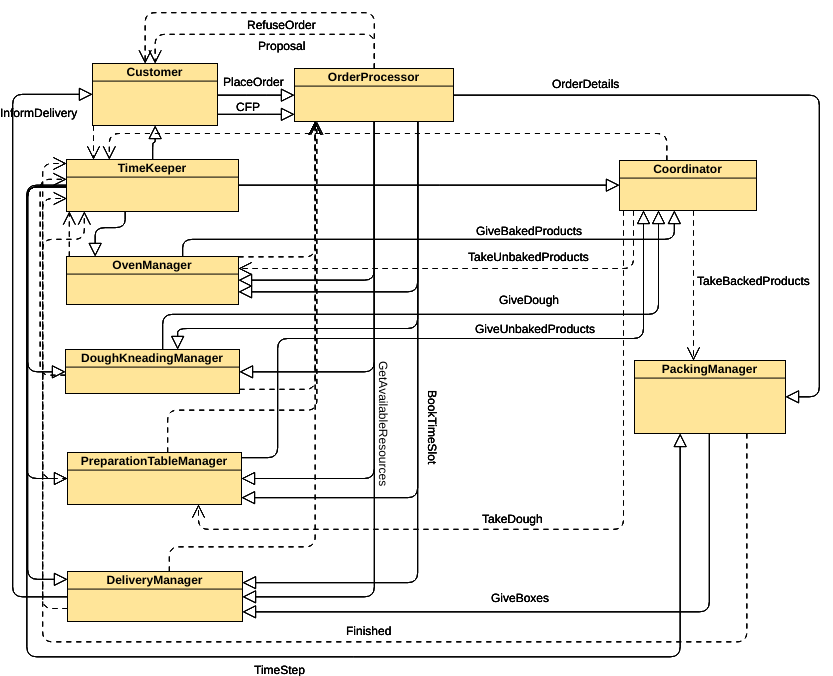
\includegraphics[width=1.0\linewidth]{Bakery.png}
    \caption{Architecture diagram explaining the interaction between customer and bakery agents}\label{fig:somename}
\end{figure}

\pagebreak

\section{Agent descriptions}%
\label{sec:agent_descriptions}

\subsection{Customer}%
\label{sub:customer_agent}
\begin{itemize}
    \item \textbf{Stage}: Order
    \item \textbf{Agent/Object}: Agent
    \item \textbf{Static/Dynamic}: Static
    \item \textbf{Behaviour}: PlaceOrder
    \item \textbf{Messages in}:
        \begin{itemize}
            \item AskForPriceProposalResponse (Sender: OrderProcessor)
            \item AskForPriceRefuseResponse (Sender: OrderProcessor)
            \item RefuseOrderResponse (Sender: OrderProcessor)
        \end{itemize}
    \item \textbf{Messages out}:
        \begin{itemize}
            \item AskForPrice (Receiver: OrderProcessor)
            \item AcceptProposal (Receiver: OrderProcessor)
        \end{itemize}
\end{itemize}

\subsection{Order Processor}%
\label{sub:order_processor}
\begin{itemize}
    \item \textbf{Stage}: Order
    \item \textbf{Agent/Object}: Agent
    \item \textbf{Static/Dynamic}: Static
    \item \textbf{Behaviour}: CFPServer, OrderServer
    \item \textbf{Messages in}:
        \begin{itemize}
            \item AskForPrice (Sender: Customer)
            \item AcceptProposal (Sender: Customer)
        \end{itemize}
    \item \textbf{Messages out}:
        \begin{itemize}
            \item AskForPriceProposalResponse (Receiver: Customer)
            \item AskForPriceRefuseResponse (Receiver: Customer)
            \item RefuseOrderResponse (Receiver: Customer)
            \item OrderDetails (Receiver: PackagingManager)
        \end{itemize}
\end{itemize}

\subsection{Oven Manager}%
\label{sub:over_manager}
\begin{itemize}
    \item \textbf{Stage}: OrderProcessing
    \item \textbf{Agent/Object}: Agent
    \item \textbf{Static/Dynamic}: Static
    \item \textbf{Behaviour}: TBD
\end{itemize}

\subsection{Dough Kneading Manager}%
\label{sub:knead_manager}
\begin{itemize}
    \item \textbf{Stage}: OrderProcessing
    \item \textbf{Agent/Object}: Agent
    \item \textbf{Static/Dynamic}: Static
    \item \textbf{Behaviour}: TBD
\end{itemize}

\subsection{Idle Time Manager}%
\label{sub:idle_manager}
\begin{itemize}
    \item \textbf{Stage}: OrderProcessor
    \item \textbf{Agent/Object}: Agent
    \item \textbf{Static/Dynamic}: Static
    \item \textbf{Behaviour}: TBD
\end{itemize}

\subsection{Dough Preparation Manager}%
\label{sub:prep_manager}
\begin{itemize}
    \item \textbf{Stage}: OrderProcessing
    \item \textbf{Agent/Object}: Agent
    \item \textbf{Static/Dynamic}: Static
    \item \textbf{Behaviour}: TBD
\end{itemize}

\subsection{Packaging Manager}%
\label{sub:packaging_manager}
\begin{itemize}
    \item \textbf{Stage}: OrderProcessing
    \item \textbf{Agent/Object}: Agent
    \item \textbf{Static/Dynamic}: Static
    \item \textbf{Behaviour}: TBD
\end{itemize}

\subsection{Delivery Manager}%
\label{sub:delivery_manager}
\begin{itemize}
    \item \textbf{Stage}: Delivery
    \item \textbf{Agent/Object}: Agent
    \item \textbf{Static/Dynamic}: Static
    \item \textbf{Behaviour}: TBD
\end{itemize}

\subsection{Time Keeper}%
\label{sub:time_keeper}
\begin{itemize}
    \item \textbf{Stage}: Order, OrderProcessing, Delivery
    \item \textbf{Agent/Object}: Agent
    \item \textbf{Static/Dynamic}: Static
    \item \textbf{Behaviour}: TBD
\end{itemize}

\subsection{Order}%
\label{sub:order}
\begin{itemize}
    \item \textbf{Stage}: Order
    \item \textbf{Agent/Object}: Object
    \item \textbf{Static/Dynamic}: Dynamic
\end{itemize}

\subsection{Truck}%
\label{sub:truck}
\begin{itemize}
    \item \textbf{Stage}: Delivery
    \item \textbf{Agent/Object}: Object
    \item \textbf{Static/Dynamic}: Static
\end{itemize}

\subsection{Product}%
\label{sub:product}
\begin{itemize}
    \item \textbf{Stage}: Order, OrderProcessing, Delivery
    \item \textbf{Agent/Object}: 
    \item \textbf{Static/Dynamic}: 
\end{itemize}

\subsection{Location}%
\label{sub:location}
\begin{itemize}
    \item \textbf{Stage}: Delivery
    \item \textbf{Agent/Object}: Object
    \item \textbf{Static/Dynamic}: Dynamic
\end{itemize}

\subsection{StreetNetwork}%
\label{sub:street_network}
\begin{itemize}
    \item \textbf{Stage}: Delivery
    \item \textbf{Agent/Object}: Object
    \item \textbf{Static/Dynamic}: Static
\end{itemize}

\section{Order Aggregation}%
\begin{itemize}
    \item As mentioned in the slides, the expected order times are as follows,
    \begin{enumerate}
    	\item 50\% to 100\% of the orders from super markets and sales shops arrive at the end of the day before delivery. They are next day orders. The remaining orders $<$ 50\% orders from the super markets and sales shops arrive on the same day as delivery.
    	\item All the orders from hospitals and old age homes arrive once a day (might not be fixed time), but for next day delivery.
    	\item Some customers like catering services, clubs etc make orders several days ahead of delivery.
    \end{enumerate}
    \item To ensure freshness and the reputation of the bakery, products can only be produced on the day of the order (however the dough preparation should also be done on the same day or not is not mentioned so we assume there is no restriction on that.)
    \item With this overview in mind we can see that before the start of the shift, the information about the next day orders is already known and hence the dough preparation can be planned for all the orders combined as it is independent of the type of product to be made.
    \item From the orders which are received (at the end of the delivery) for the super markets for the next day delivery, we can approximate them to be around 75\% ((50+100)/2) of the total orders expected and we can assume that we might get another 25\% (100-75) of orders on the same day as delivery. This is just an \textbf{estimated guess}. 
    \item In reality, it might happen that,
    \begin{enumerate}
    \item the same day orders might be less than 25\% of the total next day orders. 
    \item sometimes they might be more than 25\% of the total next day orders. 
    \end{enumerate}
    \item For the prior case, the dough is already available. For the latter case the amount of orders which are  $>$ 25\% cannot be accepted.
    \item Based on the above intuition, the order processing agent creates a work plan at the start of each shift. 
\end{itemize}


\end{document}

%\subsection{}%
%\label{sub:}
%\begin{itemize}
%    \item \textbf{Stage}: 
%    \item \textbf{Agent/Object}: 
%    \item \textbf{Static/Dynamic}: 
%    \item \textbf{Behaviour}: 
%    \item \textbf{Messages in}:
%        \begin{itemize}
%            \item msgName (Sender: sen)
%        \end{itemize}
%    \item \textbf{Messages out}:
%        \begin{itemize}
%            \item msgName (Receiver: rec)
%        \end{itemize}
%\end{itemize}
%
%
%
%\subsection{}%
%\label{sub:}
%\begin{itemize}
%    \item \textbf{Stage}: 
%    \item \textbf{Agent/Object}: 
%    \item \textbf{Static/Dynamic}: 
%\end{itemize}
